
\begin{minipage}{0.32\linewidth}
    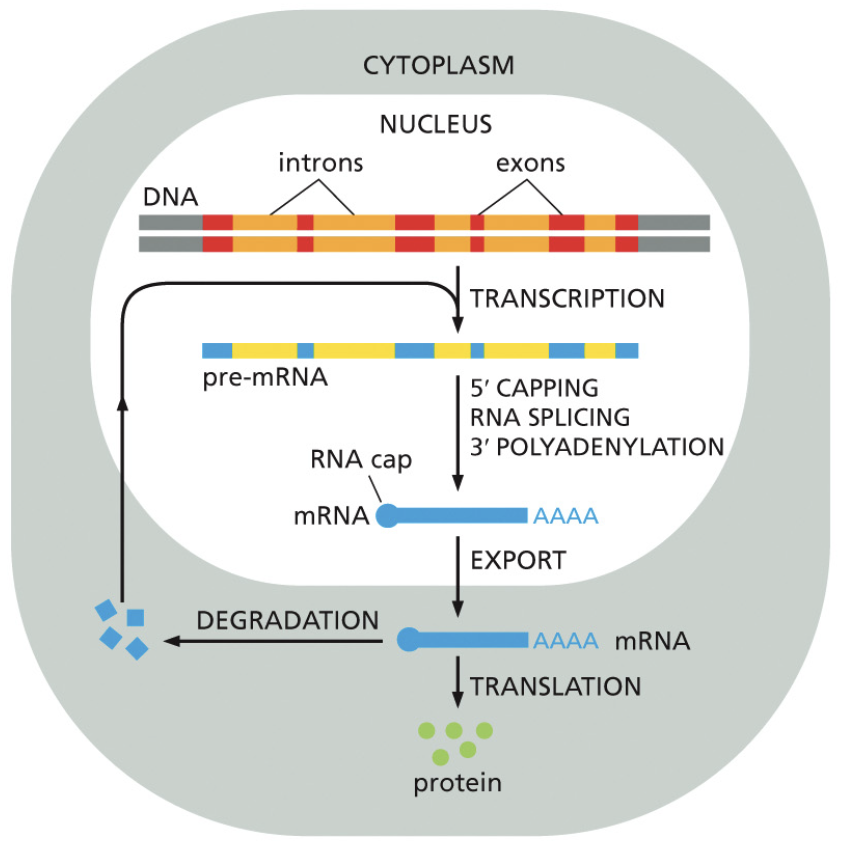
\includegraphics[width=28mm]{src/Images/eukaryot_transcription.png}\\ 
\end{minipage}
\begin{minipage}{0.68\linewidth}
\begin{itemize}
    \item Multiple types of RNA polymerases transcribe different classes of RNA.
    \item Transcription initiation is more complex.
    \item mRNA molecules undergo splicing, where introns (non-coding regions) are removed and exons (coding regions) are joined together to form the final RNA.
\end{itemize}
\end{minipage}
\hrule
\vspace{2mm}
\begin{minipage}{0.32\linewidth}
    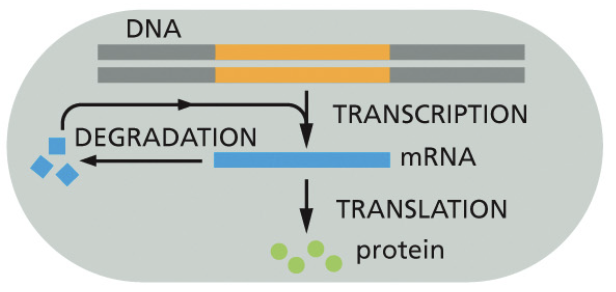
\includegraphics[width=28mm]{src/Images/prokaryot_transcription.png}\\ 
\end{minipage}
\begin{minipage}{0.68\linewidth}
\begin{itemize}
    \item 1 type of RNA polymerase transcribes all types of RNA.
    \item Transcription initiation is a simpler process.
    \item mRNA molecules are translated immediately after
transcription
\end{itemize}
\end{minipage}
\hrule
\vspace{2mm}
Both use gene regulatory proteins that bind to
specific sequences of DNA:
\begin{itemize}
    \item Repressors: Bind to sequences to turn genes off. Make it more difficult for RNA polymerase to bind to DNA.
    \item Activators: Bind to sequences to turn genes on. Make it more favorable for RNA polymerase to bind to DNA.
\end{itemize}
